\chapter{Herramientas Empleadas}\label{cap:herramientas}

En este capítulo se explican las herramientas, bibliotecas y APIs que se han utilizado en el desarrollo de AdaptaMaterialEscolar 2.0. En la Sección \ref{sec:Figma} se introduce la herramienta Figma que se ha usado para realizar el diseño de la aplicación. En la Sección \ref{sec:React} se presenta la biblioteca React que se ha empleado para implementar las interfaces de usuario de la aplicación. En la Sección \ref{sec:tailwind} se explica el framework Tailwind CSS, que se ha usado para personalizar el estilo de las páginas y los distintos elementos que las componen. En la Sección \ref{sec:Slate} se expone el framework Slate que se usa para definir el editor. En la Sección \ref{sec:Flowbite} se explica la biblioteca de componentes Flowbite que se ha utilizado para implementar de manera rápida y sencilla elementos complejos, como dropdowns. En la Sección \ref{sec:inkscape} se expone la herramienta Inkscape que se ha utilizado para crear las pautas de los ejercicios de definiciones y desarrollo. En la Sección \ref{sec:prettier} se explica la herramienta para dar formato al código fuente que se ha utilizado para mantener un estilo limpio y consistente. En la Sección \ref{sec:eslint} se presenta la herramienta ESLint que se utiliza para analizar estáticamente el código para encontrar malas prácticas y posibles errores antes de ejecutar el código.

\section{Figma}\label{sec:Figma}
Figma\footnote{\url{https://www.figma.com/}} es una herramienta web de diseño y prototipado de interfaces de usuario que ofrece una amplia gama de herramientas y recursos para crear diseños de alta calidad de manera eficiente y efectiva. Esta herramienta es especialmente útil para el diseño de aplicaciones móviles y web debido a su funcionalidad de colaboración en tiempo real y la facilidad de acceso.

Hemos empleado Figma porque nos permite crear diseños de alta fidelidad con facilidad y rapidez. Además, Figma también cuenta con una amplia variedad de recursos de diseño, como kits de interfaz de usuario y plantillas, lo que facilita aún más la creación de diseños profesionales. A eso debemos sumarle su exportabilidad, que nos permite extraer css de los diseños implementados en Figma.

En definitiva, Figma es una herramienta muy útil y efectiva para temas de diseño, debido a ello todo el diseño final de la aplicación ha sido realizado en Figma, tal y como se explicará en la Seccion \ref{subsec:DisenyoFinal}.

\section{React}\label{sec:React}
React\footnote{\url{https://es.reactjs.org/}} es una librería de JavaScript que se utiliza para crear interfaces de usuario interactivas y dinámicas en aplicaciones web. Fue desarrollada por Facebook y es una de las herramientas más populares para construir aplicaciones web modernas. En nuestra aplicación, hemos utilizado React para implementar las interfaces de usuario.

React utiliza un enfoque basado en componentes para construir interfaces de usuario, lo que significa que cada parte de la interfaz de usuario se representa como un componente. Dichos componentes son reutilizables y están diseñados para ser simples, fáciles de mantener y declarativos, es decir, describe qué se quiere hacer y no cómo hacerlo. Otras ventajas que ofrece son:

\begin{itemize}
  \item \textbf{Mayor eficiencia}: React utiliza un enfoque llamado ``reconciliación virtual'' para actualizar la interfaz de usuario de manera eficiente y minimizar el impacto en el rendimiento. Este enfoque se basa en la comparación de los estados previos y actuales de los componentes, permitiendo actualizar solo las partes necesarias de la interfaz.
  \item \textbf{Facilidad de mantenimiento}: Como se ha mencionado anteriormente los componentes de React son simples y declarativos, lo que hace que sea más fácil mantener y actualizar una aplicación web construida con React.
  \item \textbf{Biblioteca de componentes}: React tiene una gran biblioteca de componentes disponibles para su uso, lo que permite a los desarrolladores construir aplicaciones web complejas con facilidad.
\end{itemize}

Para representar las interfaces de usuario en React se utiliza una extensión de sintaxis llamada JSX que permite escribir HTML en JavaScript, lo que hace que el código sea más legible y fácil de entender. En JSX los elementos de la interfaz de usuario se definen como etiquetas HTML dentro del código JavaScript. En la Figura \ref{JSX} se muestra un ejemplo de un componente usando JSX y en la Figura \ref{SJSX} se encuentra la misma funcionalidad pero sin JSX.

\begin{figure}[ht!]

  \begin{subfigure}{\textwidth}
    \centering
    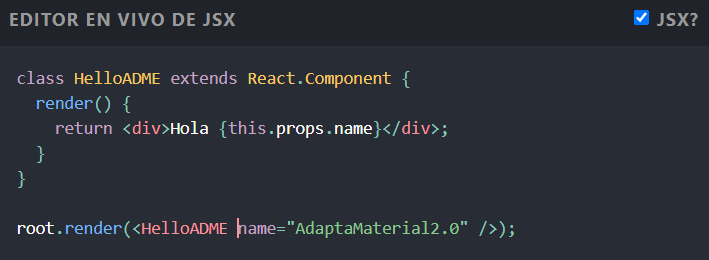
\includegraphics[width=0.6\textwidth]{Herraientas_Empleadas/ReactJSX.PNG}
    \caption{Componente con JSX.}
    \label{JSX}
  \end{subfigure}

  \begin{subfigure}{\textwidth}
    \centering
    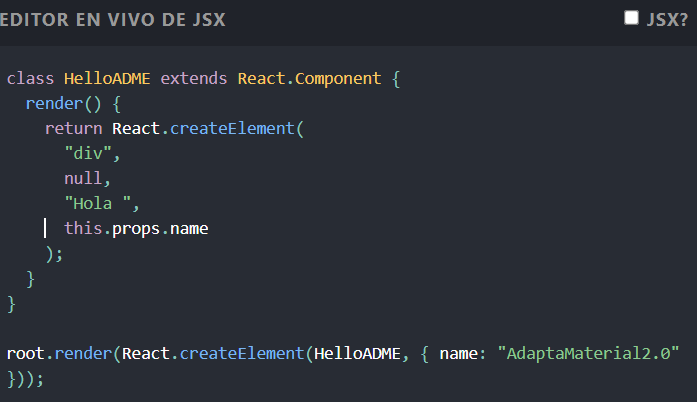
\includegraphics[width=0.6\textwidth]{Herraientas_Empleadas/ReactSinJSX.PNG}
    \caption{Componente sin JSX.}
    \label{SJSX}
  \end{subfigure}
  \caption{Componentes React}
  \label{fig:react}
\end{figure}

En los componentes de React se utiliza Tailwind CSS, una librería de estilos CSS, para la construcción rápida de interfaces de usuario sin tener que escribir CSS personalizadas para cada elemento. En la siguiente subsección se hablará de ella.

\section{Tailwind CSS}\label{sec:tailwind}
Tailwind CSS\footnote{\url{https://tailwindcss.com/}} es un framework CSS que permite aplicar estilos predefinidos directamente en el HTML sin tener que crear y manejar archivos CSS propios para conseguir un estilo concreto. Hemos decidido utilizar este framework porque facilita la labor de dar estilo al HTML de la página, debido a que no tenemos que pensar en qué clases o identificadores dar a los elementos HTML y, por lo general, tampoco necesitamos gestionar un archivo CSS por cada página o componente de React. Otra de las razones por las que hemos escogido este framework frente a otros muy parecidos, como Bootstrap\footnote{\url{https://getbootstrap.com/}}, es la facilidad que ofrece para personalizarlo y adaptarlo a nuestras necesidades. En el caso de Bootstrap, necesitas utilizar SASS o crear tus propios archivos CSS para poder personalizar el estilo, mientras que en Tailwind CSS modificando un archivo de configuración puedes personalizar/añadir colores, añadir distintos tipos de fuente de texto, añadir distintos tamaños de letra, etc. Otras ventajas que ofrece son:
\begin{itemize}
  \item \textbf{Rendimiento}: Tailwind elimina automáticamente todo el CSS que no se utilice a la hora de desplegar en producción la aplicación, consiguiendo que el paquete de CSS que se envía al cliente sea lo más pequeño posible.
  \item \textbf{Diseño responsive}: Permite aplicar distintos estilos dependiendo del tamaño de la ventana sin necesidad de usar las \textit{media queries}\footnote{\url{https://developer.mozilla.org/en-US/docs/Web/CSS/Media_Queries/Using_media_queries}} de CSS.
  \item \textbf{Reutilización}: Tailwind permite reutilizar conjuntos de utilidades que se repitan mucho definiendo una clase CSS propia que las aplique todas. Aun así, nosotros no utilizaremos, el método que ofrece Tailwind para reutilizar estilos, ya que podemos conseguir el mismo resultado creando un componente de React, con la ventaja de poder añadir lógica de JavaScript.
\end{itemize}

\section{Slate}\label{sec:Slate}
Slate\footnote{\url{https://docs.slatejs.org/}} es un framework de JavaScript de código abierto que tiene como finalidad la creación de editores de texto personalizados ``What You See Is What You Get'' (WYSIWYG). Es la herramienta ideal para este proyecto, el cual busca construir un editor de texto de alta calidad capaz de realizar diversos tipos de adaptaciones curriculares.

A diferencia de las bibliotecas de edición de texto convencionales, Slate utiliza una estructura de árbol de datos jerárquica para representar el contenido editable. En lugar de usar la estructura lineal tradicional, la estructura de árbol permite una mayor flexibilidad y personalización en la creación y edición de contenido.

El árbol de Slate está compuesto por nodos que representan diferentes tipos de contenido, como texto sin formato, texto con formato, imágenes, videos y más. Para entender mejor su estructura se explicara está en base a la Figura \ref{fig:arbolSlate}. En esta se hayan 5 nodos. El primero es todo el objeto este es el nodo documento, es decir lo que contendría la variable ``editor'', este es el contenedor de todos los demás nodos. Cada nodo hijo del nodo documento puede ser un nodo elemento o un nodo hoja.
El nodo con ``type : paragraph'' (Figura \ref{fig:arbolSlate}) es un nodo elemento de tipo bloque que da Slate por defecto. Los nodos elemento, son la capa intermedia de un documento de texto enriquecido, se puede definir nodos elemento personalizados para cualquier tipo de contenido que se desee con el estilo que se desee gracias a que este nodo permite recibir un parámetro denominado ``props''. Dentro de los nodos elemento podemos distinguir dos tipos principales de nodos elementos:

\begin{itemize}
  \item Nodo bloque: Son la opción por defecto cuando se crea un nodo elemento estos se caracterizan porque se encuentran siempre dispuestos de forma vertical ocupando todo el espacio horizontal existente.
  \item Nodo en línea: Se obtienen mediante la modificación de su comportamiento indicando al núcleo de Slate que son de tipo ``Inline'' se caracterizan por poder disponerse de forma horizontal a la vez que vertical.  El nodo con ``type: link'' (Figura \ref{fig:arbolSlate}) es de este tipo y no es propio de Slate, es decir, es creado por el desarrollador. Además, el valor "url: ..." se recibe a través del parámetro mencionado anteriormente denominado "props".
\end{itemize}

Cabe mencionar que dentro de los tipos de nodos elemento se puede diferenciar los nodos elementos editables y no editables estos se consiguen al declarase ante el núcleo de Slate como vacíos, para los no editables, porque de esta forma se considera que no hay nada en el nodo que se pueda modificar y no vacío en caso de que sean editables siendo este es el caso por defecto.
Por último, los nodos ``text : Esto es un texto'' y ``text : hyperlink'' son nodos hoja o nodos texto, son los nodos que se encuentran en el nivel más bajo del árbol y son aquellos que contienen el texto, estos no pueden tener hijos pueden contener marcas que permite enriquecer este texto, permitiendo opciones como texto en negrita, cursiva…

\begin{figure}[ht!]
  \centering
  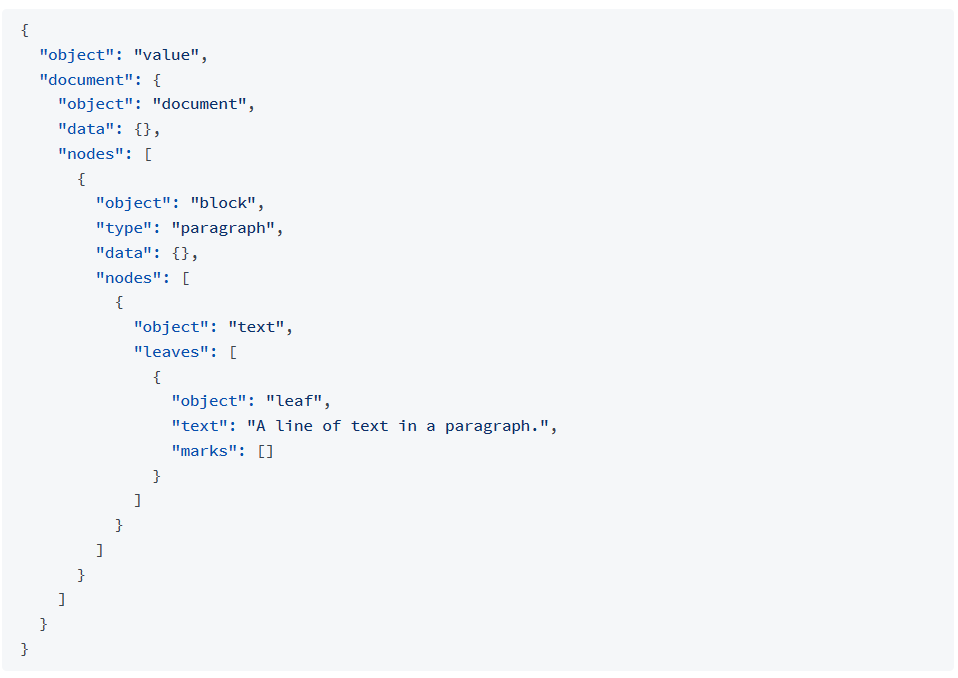
\includegraphics[width=0.8\textwidth]{Herraientas_Empleadas/ArbolSlate.png}
  \caption{Ejemplo de árbol de Slate}
  \label{fig:arbolSlate}
\end{figure}

En cuanto a las principales características de Slate, se pueden destacar:

\begin{itemize}
  \item \textbf{Personalización}: La biblioteca permite a los desarrolladores personalizar el editor de texto según sus necesidades, lo que significa que pueden definir sus propios tipos de nodos y componentes de renderizado.
  \item \textbf{Flexibilidad}: Al ser una biblioteca de JavaScript, Slate es altamente flexible y puede integrarse fácilmente con otras bibliotecas y marcos como React.
  \item \textbf{Rendimiento}: La estructura de árbol de datos utilizada por Slate permite que la biblioteca realice actualizaciones eficientes del DOM, lo que resulta en un editor de texto rápido y fluido.
  \item \textbf{Soporte de complementos}: Los complementos de Slate son módulos que proporcionan una funcionalidad adicional al editor de texto. Estos complementos pueden personalizarse y utilizarse según las necesidades del desarrollador.
  \item \textbf{Compatibilidad multiplataforma}: Slate es compatible con una amplia gama de navegadores y plataformas.
\end{itemize}

Slate es utilizado por variedad de aplicaciones web como, por ejemplo:
\begin{itemize}
  \item \textbf{Discord}: Utiliza Slate para sus canales de comunicación para colaborar y compartir.
  \item \textbf{Eraser}: Una aplicación web de borrador de fondos que utiliza Slate para permitir a los usuarios escribir y editar el texto en su sitio web.
  \item \textbf{GitBook}: Es una plataforma de creación y publicación de libros electrónicos que utiliza Slate como editor de texto para que los autores puedan escribir y editar sus libros.
\end{itemize}

\section{Flowbite}\label{sec:Flowbite}
Flowbite\footnote{\url{https://flowbite.com/}} es una librería \textit{open source} de componentes de interfaz de usuario interactivos que está desarrollada sobre Tailwind CSS. Como se ha explicado, Tailwind es una librería de CSS que se ha utilizado en el desarrollo de AdaptaMaterialEscolar 2.0, lo que hace que la integración con Flowbite sea más sencilla.

Se ha decidido utilizar esta librería principalmente ya que tiene un componente que permite hacer \textit{dropdowns} de una forma rápida y sencilla. Implementar un componente \textit{dropdown} desde cero puede ser complicado y no sería un uso eficiente del tiempo, ya que hay librerías como Flowbite que tienen componentes prediseñados.

Hemos utilizado Flowbite en funcionalidades como ejercicios de definiciones y ejercicios de desarrollo para poder seleccionar el tipo de pauta, como por ejemplo, doble pauta, cuadrícula, etc. Se usa un \textit{dropdown} que permite indicar la separación que se quiere tener entre las líneas. En el modal de la funcionalidad de pictotraductor, también se utiliza un \textit{dropdown} que permite que el usuario seleccione varias opciones. En el \textit{toolbar} del documento de trabajo, también tenemos varios \textit{dropdowns}, por ejemplo, al darle clic al botón de insertar tabla, permite seleccionar la cantidad de filas y columnas que se quiere tener. También al darle clic a los botones de cambiar color del texto y añadir color de fondo al texto, permite seleccionar los colores mediante un \textit{dropdown}.

\section{Inkscape}\label{sec:inkscape}
Inkscape\footnote{\url{https://inkscape.org/}} es un programa de código abierto y gratuito para la edición de vectores gráficos que se suele utilizar para diseñar logos, tipografías, hacer ilustraciones, etc. Se diferencia de otros programas de diseño ya que funciona con vectores, es decir, que no se trabaja con píxeles, sino que se basa en fórmulas matemáticas y esto permite ampliar la imagen sin perder calidad.

En varias funcionalidades de la aplicación el usuario tiene la opción de elegir el tipo de pauta que quiere utilizar para el ejercicio (pauta doble, pauta simple, cuadrícula, etc). El programa Inkscape se ha utilizado para crear estas pautas que se insertarán en el documento de trabajo.


\section{Prettier}\label{sec:prettier}
Prettier\footnote{\url{https://prettier.io/}} es una herramienta que permite dar formato al código de manera rápida y sencilla. Soporta muchos lenguajes, se puede integrar con la mayoría de editores de código y se pueden instalar \textit{plugins} para añadir compatibilidad con otros lenguajes o frameworks. Al ejecutarse, Prettier aplica un conjunto de reglas predefinidas para el formato del código, lo que garantiza que el código sea fácilmente legible y mantenga una apariencia uniforme, independientemente de quién lo haya escrito. Además, Prettier puede ahorrar tiempo y reducir errores humanos al automatizar la tarea de formatear el código, lo que permite que los desarrolladores se centren en escribir un código más limpio y de mayor calidad. Hay que tener en cuenta que aunque permite configurar ciertos aspectos del formato, se trata de una herramienta dogmática o inflexible, por lo tanto tiene un estilo concreto que puede no gustar a todos los usuarios.

Se ha decidido utilizar Prettier ya que es una de las herramientas para dar formato al código más utilizadas en desarrollo web y el estilo que aplica le pareció correcto a todo el equipo.

\section{ESLint}\label{sec:eslint}
ESLint\footnote{\url{https://eslint.org/}} es una de las herramientas de Linting más populares para el lenguaje de programación JavaScript. ESLint es configurable y personalizable, lo que significa que se puede adaptar para cumplir con los estándares y las necesidades específicas de cada proyecto o equipo de desarrollo. Además, ESlint puede integrarse fácilmente en los flujos de trabajo de los desarrolladores, como los sistemas de control de versiones y los editores de código, para proporcionar una retroalimentación en tiempo real sobre posibles errores o violaciones de estilo.

Se ha decidido utilizar esta herramienta por su popularidad y facilidad de uso. Se ha establecido que ESLint no tenga en cuenta errores de formato e inconsistencias de estilo, ya que de esto se encarga Prettier.

\section{API de OpenAI y GPT-3}\label{sec:openai}
La API que proporciona OpenAI\footnote{\url{https://platform.openai.com/overview}} proporciona acceso a modelos de inteligencia avanzados desarrollados por OpenAI\footnote{\url{https://openai.com/product}}. Estos modelos están diseñados para procesar y generar texto, imágenes, sonidos y otros tipos de datos. Entre ellos, se encuentra el modelo de lenguaje GPT-3, que es utilizado actualmente por ChatGPT\footnote{\url{https://openai.com/blog/chatgpt}} y puede generar texto coherente y relevante a partir de una breve descripción proporcionada por el usuario. Tanto la API de OpenAI como el modelo de lenguaje GPT-3 se han utilizado para implementar la funcionalidad de generar resumen.

Para poder utilizar esta API se pueden realizar distintas peticiones HTTP, pero si se utiliza Node.js se puede instalar el paquete ``openai''\footnote{\url{https://www.npmjs.com/package/openai}}. Este paquete proporciona la clase OpenAIApi, la cual permite utilizar distintas funciones que realizan las peticiones HTTP necesarias. En el Listing \ref{fig:configuracionOpenAIApi} se muestra la configuración de la clase OpenAIApi. La función ``createChatCompletion'' permite simular un chat con un modelo de procesamiento de texto. Esta función recibe como entrada el modelo que se quiere utilizar, y una lista de mensajes. Cada mensaje esta compuesto por el rol del autor (\textit{system}, \textit{assistant} y \textit{user}) y el contenido del mensaje (\textit{prompt}). La función ``createChatCompletion'' devuelve un objeto con información sobre la conversación y las distintas respuestas generadas a partir de los mensajes que se han enviado.

\begin{lstlisting}[label=fig:configuracionOpenAIApi, caption=Configuración de la clase OpenAIApi., language=JavaScript]
  const { Configuration, OpenAIApi} = require("openai");

  const configuration = new Configuration({
    apiKey: "Clave de la API (se necesita una cuenta de OpenAI)."
  });

  const openai = new OpenAIApi(configuration);
\end{lstlisting}